\documentclass[t,handout]{beamer}

\mode<handout>
{
  \usepackage{pgf}
  \usepackage{pgfpages}

\pgfpagesdeclarelayout{4 on 1 boxed}
{
  \edef\pgfpageoptionheight{\the\paperheight} 
  \edef\pgfpageoptionwidth{\the\paperwidth}
  \edef\pgfpageoptionborder{0pt}
}
{
  \pgfpagesphysicalpageoptions
  {%
    logical pages=4,%
    physical height=\pgfpageoptionheight,%
    physical width=\pgfpageoptionwidth%
  }
  \pgfpageslogicalpageoptions{1}
  {%
    border code=\pgfsetlinewidth{2pt}\pgfstroke,%
    border shrink=\pgfpageoptionborder,%
    resized width=.5\pgfphysicalwidth,%
    resized height=.5\pgfphysicalheight,%
    center=\pgfpoint{.25\pgfphysicalwidth}{.75\pgfphysicalheight}%
  }%
  \pgfpageslogicalpageoptions{2}
  {%
    border code=\pgfsetlinewidth{2pt}\pgfstroke,%
    border shrink=\pgfpageoptionborder,%
    resized width=.5\pgfphysicalwidth,%
    resized height=.5\pgfphysicalheight,%
    center=\pgfpoint{.75\pgfphysicalwidth}{.75\pgfphysicalheight}%
  }%
  \pgfpageslogicalpageoptions{3}
  {%
    border code=\pgfsetlinewidth{2pt}\pgfstroke,%
    border shrink=\pgfpageoptionborder,%
    resized width=.5\pgfphysicalwidth,%
    resized height=.5\pgfphysicalheight,%
    center=\pgfpoint{.25\pgfphysicalwidth}{.25\pgfphysicalheight}%
  }%
  \pgfpageslogicalpageoptions{4}
  {%
    border code=\pgfsetlinewidth{2pt}\pgfstroke,%
    border shrink=\pgfpageoptionborder,%
    resized width=.5\pgfphysicalwidth,%
    resized height=.5\pgfphysicalheight,%
    center=\pgfpoint{.75\pgfphysicalwidth}{.25\pgfphysicalheight}%
  }%
}


  \pgfpagesuselayout{4 on 1 boxed}[a4paper, border shrink=5mm, landscape]
  \nofiles
}

%% Language and font encodings
\usepackage[english]{babel}
\usepackage[utf8x]{inputenc}
\usepackage[T1]{fontenc}

\usetheme{Madrid}
\usecolortheme{beaver}

%% Useful packages
\usepackage{amsmath}
\usepackage{graphicx}

\usepackage{enumitem}

% full page itemieze
\newenvironment{fpi}
  {\itemize[nolistsep,itemsep=\fill]}
  {\vfill\enditemize}

\title{Transformations of Functions and \\
Exponential Functions}
\date{January 24, 2017}

\begin{document}
\frame{\titlepage}


\begin{frame}{Review of Section 1.2}
\begin{fpi}
\item Reminder: Week-in-Review, Help Sessions, Office Hours
\item Mathematical Models
\item Linear Regression
\item Function classes
\end{fpi}
\end{frame}

\begin{frame}{Review of Section 1.2}
Alice's parents recorded her height every 3 years when she was a child.
Find the linear regression.  Estimate her height at age 8.
\begin{table}
\begin{tabular}{c c}
Age (years) & Height (in) \\
\hline
3 & 36 \\
6 & 42 \\
9  & 48 \\
12 & 60
\end{tabular}
\end{table}

\end{frame}

\begin{frame}{Review of Section 1.2}
Classify the function as polynomial, power, rational, algebraic, trigonometric, exponential, or logarithmic.
\end{frame}

\begin{frame}{Review of Section 1.2}
Classify the function as polynomial, power, rational, algebraic, trigonometric, exponential, or logarithmic.
\end{frame}

\begin{frame}{Outline of Section 1.3 (New Functions from Old)}
\begin{fpi}
\item Vertical and horizontal shifts
\item Vertical and horizontal stretching
\item Composition
\item Commonly seen classes of functions
\end{fpi}
\end{frame}

\begin{frame}{Horizontal shifts}
To shift the graph of $y = f(x)$ to the left by $a$ units, use
$$y = f(x - a)$$
\end{frame}

\begin{frame}{Horizontal shifts}
To shift the graph of $y = f(x)$ to the right by $a$ units, use
$$y = f(x + a)$$
\end{frame}

\begin{frame}{Vertical shifts}
To shift the graph of $y = f(x)$ up by $a$ units, use
$$y = f(x) +  a$$
\end{frame}

\begin{frame}{Vertical shifts}
To shift the graph of $y = f(x)$ down by $a$ units, use
$$y = f(x) - a$$
\end{frame}

\begin{frame}{Question}
Why is the sign reversed for horizontal shifts?
\end{frame}

\begin{frame}{Horizontal stretching}
To stretch the graph of $y = f(x)$ out horizontally by a factor $c$, use
$$y = f(x/c)$$
\end{frame}

\begin{frame}{Vertical stretching}
To stretch the graph of $y = f(x)$ out vertically by a factor $c$, use
$$y = cf(x)$$
\end{frame}

\begin{frame}{Question}
Why do you divide by $c$ for horizontal stretching?
\end{frame}

\begin{frame}{Reflection across the $y$-axis}
To reflect the graph of $y = f(x)$ across the $y$ axis, use
$$y = f(-x)$$
\end{frame}

\begin{frame}{Reflection across the $x$-axis}
To reflect the graph of $y = f(x)$ across the $x$ axis, use
$$y = -f(x)$$
\end{frame}

\begin{frame}{Important note}
Remember: To reflect across the \textbf{x}-axis, multiply the \textbf{y}-value by $-1$.
To reflect across the \textbf{y}-axis, multiply the \textbf{x}-value by $-1$
\end{frame}

\begin{frame}{Summary}
\vfill
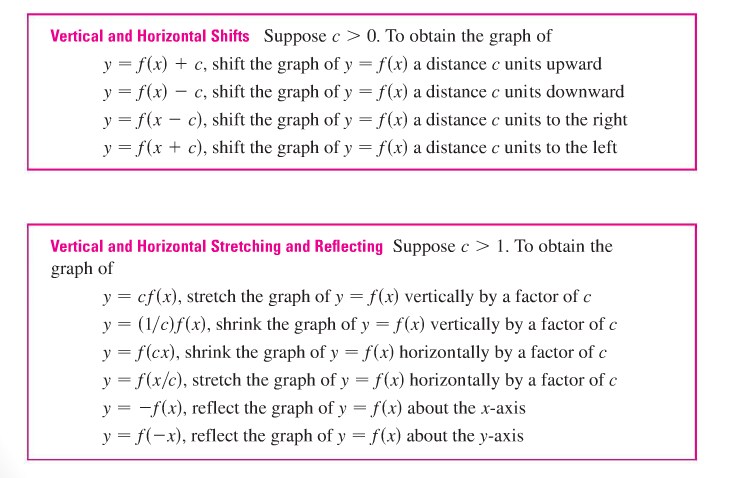
\includegraphics[width=\textwidth,height=\textheight,keepaspectratio]{shifts}
\vfill
\end{frame}

\begin{frame}{Function composition}
\begin{itemize}
\item The composition $(f \circ g)(x)= f(g(x))$ means plugging $g(x)$ into $f(x)$
\item Think of functions like machines
\end{itemize}
\vfill
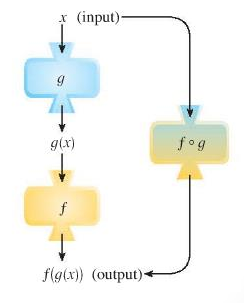
\includegraphics[width=\textwidth,height=0.5\textheight,keepaspectratio]{machines}
\vfill
\end{frame}

\begin{frame}{Function composition}
Example:
$$ f(x) = \sin(x), \qquad g(x) = x^2 + \frac{1}{x}$$
\end{frame}

\begin{frame}{Function composition}
Example:
$$ f(x) = \sqrt{x+1}, \qquad g(x) = \frac{x+1}{x-1},  \quad h(x) = x^{9}$$
\end{frame}


\begin{frame}{Function composition}
Example:
$$ f(x) = \sin^2(x +2)$$
Find a functions $g,h,k$ such that $f = g \circ h \circ k$.
\end{frame}

\begin{frame}{Function composition}
Example:
$$ f(x) = -2x^2 + 2x - 1, \qquad g(x) = -2x + 1$$
Find a function $h(x)$ such that $(g \circ h)(x) = f(x)$
\end{frame}

\begin{frame}{Function composition}
Example:
$$ f(x) = x^2 -4x + 1, \qquad g(x) = -x + 2$$
Find a function $h(x)$ such that $(h \circ g)(x) = f(x)$
\end{frame}

\begin{frame}{Function composition}
Example:
$$ f(x) = 3x^2 +6x -2, \qquad g(x) = 3x + 1$$
Find a function $h(x)$ such that $(g \circ h)(x) = f(x)$
\end{frame}


\begin{frame}{Domain review}
Find the domain of $$f(x) = \log(2 - \sqrt{x + 1})$$.
\end{frame}

\begin{frame}{Outline of Section 1.5}
\begin{fpi}
\item Exponential functions
\item Rules for manipulating exponential functions
\item Applications: Exponential growth and decay
\item Compound interest
\item Rate of growth of exponential functions
\end{fpi}
\end{frame}


\begin{frame}{Exponential functions revisited}
\begin{block}{Recall}
An \textbf{exponential function} is a function of the form
$$f(x) = a^x,$$
where $a$ is a postive constant.
\end{block}
\end{frame}

\begin{frame}{Exponential rules}
\begin{block}{Exponential rules}
If $a$ and $b$ are positive numbers then,
$$a^{x+y} = a^x a^y \qquad a^{x-y} = \frac{a^x}{a^y}  \qquad (a^x)^y = a^{xy} \qquad (ab)^x = a^x b^x$$
\end{block}
\end{frame}

\begin{frame}{Exponential rules}
\begin{fpi}
\item $3^0$
\item $81^{1/2}$
\item $8^{4/3}$
\item $4^{-1/2}$
\item $5^3 \cdot 5^{-5}$
\end{fpi}
\end{frame}

\begin{frame}{Exponential rules}
\begin{fpi}
\item $(3^2)^3$
\item $7^2 \cdot 4^2$
\item $(2 + 3)^2$
\item $\sqrt{4 + 9}$
\end{fpi}
\end{frame}

\begin{frame}{Exponential rules}
Simplify the expression
$$(4x^6)^{-1/2} \cdot x^2$$
\end{frame}

\begin{frame} {Exponential decay}
The half-life of Carbon-14 is 5730 years.  If a sample initially
contains 5mg of Carbon-14 at time $t=0$, calculate the amount
of Carbon-14 in the sample at an arbitrary time $t \ge 0$.
\end{frame}

\begin{frame} {Exponential growth}
Suppose that a population of bacteria doubles every two hours, and the initial
population of a sample is 300.  Find the population of the sample 5 hours later.
\end{frame}

\begin{frame} {Exponential growth}
A country has an annual population growth rate of 3\%. Assuming exponential growth, how many
years will it take for the population to double?
\end{frame}

\begin{frame}{Converting to base $e$}
Convert the equation $P = 121 (0.89)^t$ to the form $P = P_0 e^{kt}$.
\end{frame}

\begin{frame}{Compound Interest}
If $P$ dollars are invested at an annual rate $r$ compounded $n$ times per year, then the 
amount accumulated after $t$ years is
$$A(t) = P (1 + \frac{r}{n})^{nt}$$
\end{frame}

\begin{frame}{Continuously compounded Interest}
If $P$ dollars are invested at an annual rate $r$ compounded continuously, then the 
amount accumulated after $t$ years is
$$A(t) = P e^{rt}$$
\end{frame}


\begin{frame}{Rate of growth of exponential functions}
Out of all the function classes we've discussed so far, exponential functions of positive
base grow the fastest. 
\end{frame}

\end{document}
